\documentclass{report} 

\usepackage[italian]{babel}
\usepackage[T1]{fontenc}
\usepackage[utf8]{inputenc}
\usepackage{hyperref, listings, float, natbib, amsmath, graphicx}
\usepackage[dvipsnames]{xcolor}

\usepackage[nottoc]{tocbibind}
\usepackage[binary-units=true]{siunitx}

\definecolor{codegreen}{rgb}{0,0.6,0}
\definecolor{codegray}{rgb}{0.5,0.5,0.5}
\definecolor{codepurple}{rgb}{0.58,0,0.82}
\definecolor{backcolour}{rgb}{0.95,0.95,0.92}

\lstdefinestyle{mycode}{
    backgroundcolor=\color{backcolour},   
    commentstyle=\color{codegreen},
    keywordstyle=\color{magenta},
    numberstyle=\tiny\color{codegray},
    stringstyle=\color{codepurple},
    basicstyle=\ttfamily\footnotesize,
    breakatwhitespace=false,         
    breaklines=true,                 
    captionpos=b,                    
    keepspaces=true,                 
    numbers=left,                    
    numbersep=5pt,                  
    showspaces=false,                
    showstringspaces=false,
    showtabs=false,                  
    tabsize=2
}

\lstset{style=mycode}

\title{Rust Safeness}
\author{Edoardo De Matteis}

\begin{document}

\maketitle
\tableofcontents

\clearpage 

\chapter{Introduzione} \label{sec:politica_di_sicurezza}
Il linguaggio di programmazione \textit{Rust} è noto e apprezzato principalmente per la sua efficienza computazionale e per le sue garanzie sulla sicurezza ~\cite[1]{rust:rustonomicon}, a tal proposito è molto difficile parlare di sicurezza in generale dato che non ne esiste una definizione assoluta, è un concetto relativo che varia in base a cosa ci interessa proteggere e garantire. La sicurezza di un'organizzazione - che essa sia una multinazionale o un singolo individuo - è definita da una \textbf{security policy}: un documento contenente regole, principi e pratiche che determinano come garantire che il sistema si trovi in uno stato sicuro ~\cite{milner:type_polymorphism}. Nell'ambito della sicurezza informatica con l'avvento di internet e la sempre più grande condivisione di codice è nata la necessità di verificare la sicurezza di programmi e per estensione dei linguaggi di programmazione, per dimostrare delle proprietà di un linguaggio è necessario avere una definizione formale della sua \textbf{semantica} ovvero l'insieme delle regole che definiscono il significato di un linguaggio e dei suoi programmi. \\
In \textit{Rust} un programma è sicuro se rispetta \textbf{memory safety} (capitolo \ref{chap:memory_safety}) e \textbf{semantica statica} (capitolo \ref{chap:type_safety}) ~\cite[14]{rust:reference} ma la documentazione presenta delle definizioni poco chiare se non addirittura contraddittorie:

\begin{center}
    "Rust code is incorrect if it exhibits any of the behaviors in the following list. This includes code within \colorbox{backcolour}{\texttt{unsafe}} blocks and \colorbox{backcolour}{\texttt{unsafe}} functions. \colorbox{backcolour}{\texttt{unsafe}} only means that avoiding undefined behavior is on the programmer; it does not change anything about the fact that Rust programs must never cause undefined behavior. [...] There is no formal model of Rust's semantics for what is and is not allowed in unsafe code" ~\cite[14.3]{rust:reference}
\end{center}

L'uso del termine "unsafe" è causa di confusione dal momento che \colorbox{backcolour}{\texttt{unsafe}} è un costrutto sintattico che consente la scrittura di codice che può causare \textbf{undefined behavior}, per questo si dice che Rust è composto da due "sottolinguaggi": \textit{unsafe Rust} e \textit{safe Rust} in base alla presenza o meno di un blocco \colorbox{backcolour}{\texttt{unsafe}}, questo costrutto è desiderabile perché permette sia di poter comunicare con librerie in \textit{C} che di avere un accesso più esplicito alla memoria ~\cite[1.2]{rust:rustonomicon}. \\ 
Piuttosto che una definizione formale di undefined behavior si ha una lista in continuo aggiornamento ~\cite[14.3]{rust:reference}. 
Nella citazione riportata sono presenti fonti di confusione: nella stessa frase viene detto prima che in un blocco \colorbox{backcolour}{\texttt{unsafe}} sia compito del programmatore evitare undefined behavior e subito dopo viene affermato come le garanzie sulla safety siano le stesse di un blocco \colorbox{backcolour}{\texttt{safe}}, quindi anche l'assenza di undefined behavior. Volendo comunque considerare solo l'ultima affermazione, l'esecuzione in un blocco \colorbox{backcolour}{\texttt{unsafe}} di uno degli esempi in lista non dovrebbe causare undefined behavior; nel listato \ref{lst:unsafe_raw} si ha un \textbf{raw pointer dereferencing} (presente in lista come dimostrato in figura \ref{fig:warning}): dato un puntatore riesco a leggere il dato memorizzato nella locazione puntata tramite l'aritmetica dei puntatori tipica del C. È ragionevole che in unsafe Rust questo sia possibile ma mette in luce come la documentazione sia poco chiara. 

\lstinputlisting{../code/Unsafe/raw.rs}
\lstinputlisting[caption={Raw pointer dereferencing in un blocco \texttt{unsafe}}, label={lst:unsafe_raw}]{../code/Unsafe/output/rawrs.txt}

\begin{figure}[h!t]
    \centering
    \label{fig:warning}
    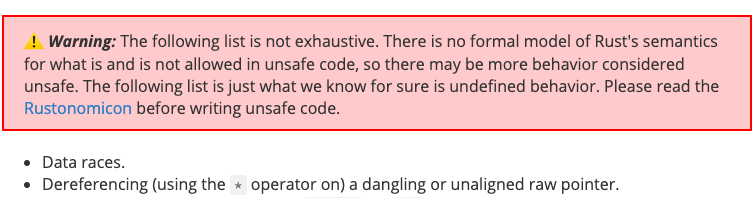
\includegraphics[scale=0.45]{images/warning_undefined_behavior.png}
    \caption{Il raw pointer dereferencing è considerato undefined behavior}
\end{figure}

\chapter{Memory Safety} \label{chap:memory_safety}

\section{Configurazione della memoria}
Consideriamo tre diversi tipi di allocazione della memoria presenti nei linguaggi C e Rust:
\begin{itemize}
    \item \textbf{Allocazione statica}. Il compilatore memorizza solo ed esclusivamente le variabili globali, il nome deriva dal fatto che in C una variabile in una funzione è dichiarata globalmente tramite la keywork \colorbox{backcolour}{\texttt{static}}.
    
    \item \textbf{Allocazione automatica}. Se durante l'esecuzione del codice è possibile sapere in anticipo quanta memoria dovrà  essere allocata si esegue allocazione automatica tramite una struttura dati detta \textbf{stack} o \textbf{call stack}, la cui particolarità è quella di crescere verso il basso; alcune entità che richiedono allocazione automatica sono le variabili di tipo primitivo e le funzioni. Sia con l'allocazione statica che automatica la memoria da allocare è nota già a tempo di compilazione, la sequenza delle operazioni però è nota solo durante l'esecuzione e questo giustifica la necessità di questo secondo tipo di allocazione. 
    
    \item \textbf{Allocazione dinamica}. Per oggetti la cui dimensione non è prevedibile (come tipi composti o liste dinamiche) si usa una struttura dati nota come \textbf{heap} che ha la particolarità di crescere verso l'alto. Proprio a causa del fatto che heap e stack crescono in direzioni opposte si può causare un \textbf{overflow} (sezione \ref{sec:buffer_overflow}). Ad ogni modo quando si chiama una funzione che usa una struttura dinamica nello stack viene salvato il puntatore di tale struttura esplicitamente in linguaggi come il C, all'insaputa del programmatore in \textit{Java} ed esplicitamente in Rust ma con dei controlli che evitano comportamenti non sicuri.  
\end{itemize}

Questo approccio è stato reso popolare dal C ed è oggi adottato da numerosi linguaggi, sempre in C esiste un ulteriore tipo di allocazione della memoria noto come \textbf{register allocation} che permette di scrivere direttamente su un blocco del processore; non essendo presente in Rust non viene approfondita. \\

\section{Violazione della memory safety}
Definiamo un'entità software \textbf{memory safe} quando non accede ad indirizzi di memoria fuori dal proprio \textbf{address space} (una zona di memoria dedicata all'entità software sopra citata) né esegue istruzioni fuori dall'area assegnatale da compilatore e linker ~\cite{paper:def}, un linguaggio che garantisce la memory safety dei suoi programmi è detto memory safe.\\
I linguaggi in cui la gestione della memoria è lasciata al programmatore sono generalmente unsafe (come C o \textit{C++}), altri linguaggi quali Java o \textit{C\#} risolvono il problema nascondendo i puntatori e gestendo automaticamente la memoria, obbligando il linguaggio ad eseguire i dovuti controlli e spesso usando un \textbf{garbage collector} che rende nuovamente disponibile la memoria allocata. In safe Rust è presente l'aritmetica dei puntatori e non si ha garbage collector, questo è possibile grazie ai meccanismi di \textbf{ownership} (sezione \ref{sec:double_free}) e \textbf{borrowing} (sezione \ref{sec:dangling_reference}).

\subsection{Buffer Overflow} \label{sec:buffer_overflow}
Quando in un buffer si possono inserire dati di dimensione maggiore della sua capacità sovrascrivendo così altre informazioni ~\cite{nist:800} si può parlare di buffer overflow. \\
Un esempio esplicativo ed interessante di buffer overflow in C è nel listato \ref{lst:stackoverflowc} ~\cite[7.5]{stallings:os}: dato che gli array sono posizionati uno dopo l'altro (in ordine LIFO essendo dati allocati su uno stack) si riesce a leggere e scrivere su \texttt{str1} eludendo anche il controllo di uguaglianza, nel terzo caso questo controllo viene superato perché si confrontano solo i primi 8 caratteri. In Rust questo non è possibile, si veda nel listato \ref{lst:bufofrs} come il linguaggio esegua dei controlli sulle dimensioni degli array, esattamente ciò che la funzione \texttt{gets} non fa. 

\lstinputlisting{../code/BufferOverflow/StackOverflow/StackAttack/stackattack.c}
\lstinputlisting[caption={Stack overflow in C}, label={lst:stackoverflowc}]{../code/BufferOverflow/StackOverflow/StackAttack/output/stackattack_c.txt}

\lstinputlisting{../code/BufferOverflow/bufof.rs}
\lstinputlisting[caption=Buffer overflow in Rust, label={lst:bufofrs}]{../code/BufferOverflow/output/bufof_rs.txt}

\subsection{Stack Overflow}
Quando si chiama una funzione si salva lo \textbf{stack frame} (noto anche come \textbf{activation record} è una zona del call stack contenente dati necessari alla funzione attualmente in esecuzione) e può capitare che chiamate ricorsive facciano entrare il programma in uno stato di non terminazione, Rust individua a tempo di compilazione la ricorsione infinita e segnala l'overflow a tempo di esecuzione. In C l'errore che si vede è dato dal sistema operativo (macOS Catalina 10.15.3) perché con questa ricorsione infinita si prova ad accedere ad un frammento di memoria protetto.

\lstinputlisting{../code/BufferOverflow/StackOverflow/Recursion/recursion.c}
\lstinputlisting[caption={Stack overflow ricorsivo in C}, label={lst:recursionc}]{../code/BufferOverflow/StackOverflow/Recursion/output/recursion_c.txt}

\lstinputlisting{../code/BufferOverflow/StackOverflow/Recursion/recursion.rs}
\lstinputlisting[caption={Stack overflow ricorsivo in Rust}, label={lst:recursionrs}]{../code/BufferOverflow/StackOverflow/Recursion/output/recursion_rs.txt}

\subsection{Integer Overflow}
In qualsiasi macchina non astratta si ha memoria finita ed è rappresentabile solo un insieme finito di numeri, quando un valore è troppo grande (o piccolo) per essere rappresentato si ha un overflow. Sono due gli approcci principali per risolvere un integer overflow, ognuno basato su un'aritmetica differente:
\begin{itemize}
    \item \textbf{Modular arithmetic}. Si applica un wrapping ad ogni numero in overflow, dato il valore $n$ e una memoria a $m$ bit si memorizza $w = n \mod m$.
    \item \textbf{Saturation arithmetic}. Dati $min$ e $max$ - rispettivamente il numero più grande e più piccolo rappresentabile - e un numero $n$ in memoria viene salvato
    \begin{equation*}
        c = \begin{cases}
            max & n > max \\
            min & n < min \\
            n  & \text{altrimenti} \\
        \end{cases}
    \end{equation*}
\end{itemize}

L'integer overflow ha in passato causato problemi molto seri: durante il volo inaugurale del lanciatore \textit{Ariane 5} un integer overflow dovuto ad una conversione in intero a 16 bit di un float a 64 bit ha causato una reazione a catena per cui il razzo ha virato orizzontalmente distruggendosi poco dopo il lancio, il codice scritto in Ada non prevedeva controlli di overflow come esplicitamente richiesto dai progettisti per motivi di efficienza. In Rust si hanno due modalità di compilazione: in \textbf{debug mode} si eseguono dei controlli in più rispetto alla \textbf{release mode} tra cui controlli dinamici per l'integer overflow - listato \ref{lst:integeroverflowrs} - contrariamente al C che applica direttamente wrapping. \\
Differenti linguaggi adottano differenti approcci: se si può prevedere il valore massimo possibile in un programma allora è in generale facile evitare integer overflow; in caso contrario si possono utilizzare metodi dinamici come in Rust. 

\lstinputlisting{../code/IntegerOverflow/intof.rs}
\lstinputlisting[caption={Integer overflow in Rust}, label={lst:integeroverflowrs}]{../code/IntegerOverflow/output/intof_rs.txt}

Nel listato \ref{lst:integeroverflowc} si prende un intero come primo argomento e una stringa - idealmente di lunghezza pari al primo argomento - come secondo. Il problema sorge nella conversione da integer a short, inserendo come primo argomento 65536 ($2^{16}$ che non è rappresentabile con i soli 16 bit di uno short) si causa un buffer overflow, combinandone la pericolosità con la difficoltà di rivelamento dell'integer overflow.

\lstinputlisting{../code/IntegerOverflow/width1.c}
\lstinputlisting[caption={Integer overflow in C}, label={lst:integeroverflowc}]{../code/IntegerOverflow/output/width1_c.txt}

\subsection{Double-Free} \label{sec:double_free}
Si ha un double free error ~\cite[10.4.4]{gollmann:computersecurity} quando si prova a liberare più volte la stessa zona di memoria e in Rust non è possibile grazie all'ownership, questa rappresenta il possesso di un'area memoria e impedisce a questa di esser puntata da più puntatori, nel listato \ref{lst:doublefree_rs} si può vedere come \texttt{s1} perda validità dopo aver trasferito a \texttt{s2} l'ownership della stringa cui puntava.

\lstinputlisting{../code/DoubleFree/doublefree.rs}
\lstinputlisting[caption={Ownership}, label={lst:doublefree_rs}]{../code/DoubleFree/output/doublefree_rs.txt}

In C invece si può osservare il codice nel listato \ref{lst:doublefree_c}: si immagini di avere un servizio ad iscrizione salvando ogni utente tramite una struct \texttt{User}: Guido libera la propria memoria che, disponibile, potrà memorizzare \texttt{Luisa} che si è appena iscritta. Il puntatore \texttt{Guido} però ora punta all'account di Luisa e con \texttt{free(Guido)} proprio l'account di Luisa viene eliminato con il risultato che non solo Luisa non ha più un account ma a quello di Carla possono accedere sia Guido che Luisa.

\lstinputlisting{../code/DoubleFree/doublefree.c}
\lstinputlisting[caption={Double free in C}, label={lst:doublefree_c}]{../code/DoubleFree/output/doublefree_c.txt}

Il puntatore \texttt{Guido} è anche un \textbf{dangling pointer}.

\subsection{Dangling References} \label{sec:dangling_reference}
Quando un oggetto viene eliminato ma il suo puntatore no si ha un dangling pointer che permettere di accedere a memoria cui non dovrebbe. \\
Immaginiamo ora che per vendicarsi Luisa abbia scritto un semplice sistema di messaggistica per leggere la corrispondenza di Guido, la procedura \texttt{send\_message} crea un puntatore di tipo \texttt{Message} che ha scope solo ed esclusivamente dentro \texttt{send\_message} ma facendo riferimento esplicito a quella locazione Luisa riesce a leggere il messaggio di Guido anche dopo che questo non esiste più. Nel listato \ref{lst:dangrefc} l'indirizzo viene stampato a schermo e inserito dall'utente (indicato da "$>$") per semplicità, lo si può rendere in modo più esplicito mantenendo una variabile per il puntatore, sia essa \texttt{mess} stessa o una ad hoc passata come argomento alla funzione.

\lstinputlisting{../code/DanglingReference/dangref.c}
\lstinputlisting[caption={Dangling pointer in C}, label={lst:dangrefc}]{../code/DanglingReference/output/dangref_c.txt}

In Rust non possiamo usare i puntatori perché l'ownership ci obbliga ad avere un puntatore solo e una volta disabilitato non possiamo più accedere a quell'area di memoria né si può leggere la locazione perché non è permesso il raw dereferencing; esistonono però le reference ~\cite[4.2]{rust:language} che permettono di prendere in prestito (borrowing) una variabile senza esserne proprietari, nel listato \ref{lst:dangrefrs} \texttt{s} nella riga 5 è quindi una \textbf{shallow copy} di \texttt{s2}, se una \textbf{deep copy} è la copia di tutto il contenuto di un oggetto con una shallow copy si memorizza solo il puntatore. Come con l'ownership anche nel borrowing si ha validità solo dentro il proprio scope.

\lstinputlisting{../code/DanglingReference/dangref.rs}
\lstinputlisting[caption={Dangling reference in Rust}, label={lst:dangrefrs}]{../code/DanglingReference/output/dangref_rs.txt}

\clearpage
\chapter{Type Safety} \label{chap:type_safety}
Ogni oggetto in matematica ha un \textbf{tipo}, basti pensare al fatto che non è possibile eseguire un'operazione come $ \{13\} \land 10 $ dato che $\{13\}$ è un insieme, $10$ è un numero e $\land$ è un connettivo logico.\\
 Lo stesso vale nei linguaggi di programmazione: l'insieme delle regole che assegna un tipo ad ogni espressione è detto semantica statica o \textbf{sistema dei tipi}; volendo dare una definizione di \textbf{type safety} si tenga conto che durante l'esecuzione di un programma si può incorrere in due tipi di errori: \textbf{trapped} e \textbf{untrapped}, i primi sono facilmente riconoscibili dato che interrompono l'esecuzione, i secondi no e per questo sono molto più difficili da individuare. Un linguaggio in cui nessun programma ben tipato - nei linguaggi con \textbf{tipizzazione statica} è onere del programmatore specificare il tipo di ogni variabile, si suppone quindi che non ci siano errori durante questa fase - genera errori trapped né untrapped si dice \textbf{sound}, solo untrapped invece si dice \textbf{safe}, un linguaggio sound è necessariamente safe ~\cite{cencia:dispense}.\\ 
 Una definizione simile è quella di Milner per cui 
 \begin{center}
    \textit{well-typed programs cannot “go wrong”} ~\cite{milner:type_polymorphism}
 \end{center}
 con programmi che si "comportano male" si possono intendere programmi non sound o che generano undefined behavior (sezione \ref{sec:politica_di_sicurezza}). 

\section{Violazione della type safety}
\subsection{Type Confusion} \label{sec:type_confusion}
Nel listato \ref{lst:lilliputc} si alloca un array di short ($\SI{2}{\byte} $) staticamente, andrà quindi sullo stack e considerando che il computer su cui ho eseguito il programma monta un processore Intel - little endian- si ha la seguente rappresentazione in memoria

\begin{table}[H]
	\label{fig:mem_type_stack}
	\centering
	\begin{tabular}{|c|c|}
		\hline
		\texttt{1} & \texttt{1000000000000000} \\
		\hline 
		\texttt{0} & \texttt{0000000000000000} \\
		\hline
	\end{tabular}
\end{table}

il puntatore \texttt{p} punta al primo elemento ma essendo \texttt{int} legge $\SI{4}{\byte}$  
\[
\texttt{00000000000000001000000000000000} \\
\]
che in decimale equivale a $ 2^{16} = 65536 $.

\lstinputlisting{../code/TypeSafety/Lilliput/lilliput.c}
\lstinputlisting[caption={Type confusion in C}, label={lst:lilliputc}]{../code/TypeSafety/Lilliput/output/lilliput_c.txt}

In Rust non si può proprio puntare ad una variabile con un tipo differente da quello della variabile stessa.

\lstinputlisting{../code/TypeSafety/Lilliput/lilliput.rs}
\lstinputlisting[caption={Type confusion in Rust}, label={lst:lilliputrs}]{../code/TypeSafety/Lilliput/output/lilliput_rs.txt}

\chapter{Note al Professore}
Nella sezione \ref{sec:type_confusion} non sono riuscito a trovare esempi significativi di type confusion in C proprio grazie alla semplicità del linguaggio e assenza di classi quindi sembra più un'opacità semantica come ha detto Lei.

\clearpage
%\bibliographystyle{unsrtnat}
\bibliographystyle{plain}
\bibliography{paper}{}

\end{document}
